% !TEX program = pdflatex
% !TEX encoding = UTF-8 Unicode

% Plantilla, basada en la clase `scrbook` del paquete KOMA-script,  para la elaboración de un TFG siguiendo las directrices del la comisión del Grado en Matemáticas de la Universidad de Granada.

% Francisco Torralbo Torralbo

\documentclass[print, color]{ugrTFG}

% VERSIÓN ELECTRÓNICA PARA TABLETA
% Cambiando la opción "print" por "tablet" generaremos un pdf adaptado para leerlo en tabletas de 9 pulgadas.

% -------------------------------------------------------------------
% INFORMACIÓN DEL TFG Y EL AUTOR
% -------------------------------------------------------------------

\newcommand{\miTitulo}{Título del trabajo\xspace}
\newcommand{\miNombre}{Nombre apellidos\xspace}
\newcommand{\miGrado}{Grado en Matemáticas}
\newcommand{\miFacultad}{Facultad de Ciencias}
\newcommand{\miUniversidad}{Universidad de Granada}

% Añadir tantos tutores como sea necesario separando cada uno de ellos mediante el comando `\medskip` y una línea en blanco
\newcommand{\miTutor}{
  Nombre del tutor 1 \\ \emph{Departamento del tutor 1} 

  % Añadir tantos tutores como sea necesario. 

  \medskip
  Nombre del tutor 2 \\ \emph{Departamento del tutor 2}
}
\newcommand{\miCurso}{2023-2024\xspace}

\hypersetup{
	pdftitle={\miTitulo},
	pdfauthor={\textcopyright\ \miNombre, \miFacultad, \miUniversidad}
}

\begin{document}

\maketitle

% -------------------------------------------------------------------
% FRONTMATTER
% -------------------------------------------------------------------
\frontmatter % Desactiva la numeración de capítulos y usa numeración romana para las páginas

% !TeX root = ../tfg.tex
% !TeX encoding = utf8
%
%*******************************************************
% Declaración de originalidad
%*******************************************************

\thispagestyle{empty}

\hfill\vfill

\textsc{Declaración de originalidad}\\\bigskip

D./Dña. \miNombre \\\medskip

Declaro explícitamente que el trabajo presentado como Trabajo de Fin de Grado (TFG), correspondiente al curso académico \miCurso, es original, entendido esto en el sentido de que no he utilizado para la elaboración del trabajo fuentes sin citarlas debidamente.
\medskip

En Granada a \today 
\vspace{3cm}
\begin{center} 
	\begin{figure}[H]
		\center
		
\includegraphics[width=35mm]{img/firma.jpeg}
	\end{figure}
	
Fdo: \miNombre 

\end{center}

\vfill

\cleardoublepage
\endinput
   
% !TeX root = ../tfg.tex
% !TeX encoding = utf8

%*******************************************************
% Dedication
%*******************************************************
\thispagestyle{empty}
\phantomsection 
\pdfbookmark[1]{Dedicatoria}{Dedicatoria}

\hfill
\vfill

\begin{flushright}
\itshape
A mi familia y amigos, \\
y en especial a Inés.
\end{flushright}

\vfill

\cleardoublepage
\endinput
                % Opcional
% !TeX root = ../tfg.tex
% !TeX encoding = utf8

%*******************************************************
% Table of Contents
%*******************************************************
\phantomsection
\pdfbookmark[0]{\contentsname}{toc}

\setcounter{tocdepth}{2} % <-- 2 includes up to subsections in the ToC
\setcounter{secnumdepth}{3} % <-- 3 numbers up to subsubsections

\tableofcontents 

%*******************************************************
% List of Figures and of the Tables
%*******************************************************

    % *******************************************************
    %  List of Figures
    % *******************************************************    
    \phantomsection 
    % \listoffigures

    %*******************************************************
    % List of Tables
    %*******************************************************
    \phantomsection 
    % \listoftables
    
    %*******************************************************
    % List of Listings
    % The package \usepackage{listings} is needed
    %*******************************************************      
	  % \phantomsection 
    % \renewcommand{\lstlistlistingname}{Listados de código}
    % \lstlistoflistings 

\cleardoublepage
            
% !TeX root = ../tfg.tex
% !TeX encoding = utf8

%*******************************************************
% Agradecimientos
%*******************************************************

\chapter{Agradecimientos}

Quisiera comenzar agradeciendo a mis tutores, Miguel y Julián, por su gran ayuda
y dedicación en todo momento de este trabajo.
\bigskip

A mis padres y hermanos, así como a mis abuelos, por apoyarme de manera
incondicional desde la distancia y no dejar que me rindiera.
\bigskip

También quisiera agradecer a todos aquellos compañeros y amigos que, de una forma
u otra, me han ayudado con este trabajo tanto con sus ideas y opiniones como con
su aliento.
\bigskip

Por último, quisiera agradecérselo a Inés. Por tu paciencia y tu apoyo continuo,
por estar a mi lado cuando más lo necesitaba, gracias.

\cleardoublepage
\endinput            % Opcional

% !TeX root = ../tfg.tex
% !TeX encoding = utf8
%
%*******************************************************
% Summary
%*******************************************************

\selectlanguage{english}
\chapter{Abstract}

This Bachelor's Thesis explores the integration of Topological Data Analysis (TDA)
with convolutional neural networks (CNNs) to clarify and enhance our
understanding of how CNNs manipulate data. Given the common perception of CNNs as
\enquote{black boxes} due to the opacity on their internal decision-making
processes, this work adopts an alternative approach through the application of persistent
homology techniques, a key tool in TDA. This allows for a detailed analysis of the
data structure during CNN processing, facilitating greater transparency and
understanding of these networks' internal workings from a topological point of view.

The study focuses on the applicability of persistent homology to provide an additional
layer of explainability and optimization to deep learning models. The underlying
theory is explored, and implementations are carried out in practical cases using
advanced network architectures such as ResNet, EfficientNet and DenseNet. Through
controlled experiments, it is demonstrated that topological regulation not only
improves the performance of CNNs in image classification and transfer learning
tasks, but also offers new insights into the data structure throughout the learning
process.

Specific results indicate that different configurations in CNN models significantly
influence the topological characteristics of the data. The dynamics of the
architectures studied show an initial tendency to simplify the data, possibly to
remove noise and irrelevant details. However, as learning progresses, the
topological complexity of the data increases, suggesting a deliberate strategy to
develop richer and more detailed representations, thereby facilitating better
differentiation between classes.

The implementation of a topological regularizer in selected models such as
EfficientNet-B0 and DenseNet-121 has proven to be particularly promising. This approach
adjusts the topological complexity of the data in a way that reflects a significant
improvement in the accuracy and efficacy of classification. Moreover, it is observed
that knowledge transfer markedly improves when the data topology is appropriately
manipulated, suggesting that topological modifications could be an effective
strategy for optimizing CNNs.

In conclusion, this document not only enhances the understanding of CNNs'
internal mechanisms through TDA but also marks a step towards more transparent
and reliable artificial intelligence (AI) models. The findings shows the utility
of TDA in the field of deep learning, proposing a new alternatives for
explainability and efficiency that may be interesting to consider in the future
evolution of computer vision and data science.

\bigskip
\textbf{Keywords}: convolutional neural networks, topological data analysis,
persistent homology, AI explainability, optimization of deep learning models, transfer
learning.

% Al finalizar el resumen en inglés, volvemos a seleccionar el idioma español para el documento
\selectlanguage{spanish}
\chapter{Resumen}

Este Trabajo de Fin de Grado (TFG) explora la integración del Análisis de Datos
Topológico (TDA) con redes neuronales convolucionales (CNNs) para clarificar y
mejorar nuestra comprensión de cómo las CNNs manipulan los datos. Dada la percepción
común de las CNNs como \enquote{cajas negras} debido a la opacidad en sus
procesos de toma de decisiones internos, este trabajo adopta un enfoque alternativo
mediante la aplicación de técnicas de homología persistente, una herramienta
clave en TDA. Esto permite un análisis detallado de la estructura de datos durante
el procesamiento en las CNNs, facilitando una mayor transparencia y
entendimiento de los mecanismos internos de estas redes desde un punto de vista
topológico.

El estudio se centra en la aplicabilidad de la homología persistente para
proporcionar una mayor explicabilidad y optimización de los modelos de
aprendizaje profundo. Se explora la teoría matemática subyacente, para
posteriormente realizar implementaciones en casos prácticos utilizando
arquitecturas de CNNs avanzadas como ResNet, EfficientNet y DenseNet. A través
de experimentos controlados, se demuestra que la regulación topológica no solo mejora
el rendimiento de las CNNs en tareas de clasificación de imágenes y de transferencia
de conocimiento, sino que también ofrece nuevas perspectivas sobre la estructura
de los datos a lo largo del proceso de aprendizaje.

Los resultados indican que las diferentes configuraciones en los modelos de CNNs
influyen significativamente en las características topológicas de los datos. La dinámica
de las arquitecturas estudiadas muestra una tendencia inicial a simplificar los datos,
posiblemente para eliminar ruido y detalles irrelevantes. Sin embargo, a medida
que avanza el aprendizaje, la complejidad topológica de los datos aumenta,
sugiriendo una estrategia deliberada para obtener representaciones más ricas y
detalladas, facilitando así una mejor diferenciación entre clases.

La implementación de un regularizador topológico en modelos como EfficientNet-B0
y DenseNet-121 ha demostrado ser particularmente prometedora. Este enfoque
ajusta la complejidad topológica de los datos de manera que refleja una mejora
significativa en la precisión y eficacia de la clasificación. Además, se observa
que la transferencia de conocimiento mejora considerablemente cuando la
topología de los datos se manipula adecuadamente, sugiriendo que las modificaciones
topológicas podrían ser una estrategia efectiva para optimizar las CNNs.

En conclusión, este documento no solo mejora la comprensión de los mecanismos
internos de las CNNs a través de TDA, sino que también marca un paso hacia modelos
de inteligencia artificial (IA) más transparentes y confiables. Los hallazgos
destacan la utilidad del TDA en el campo del aprendizaje profundo, proponiendo nuevas
alternativas para la explicabilidad y eficiencia que pueden ser interesantes de considerar
en la evolución futura de la visión artificial y la ciencia de datos.

\bigskip
\textbf{Palabras clave}: redes neuronales convolucionales, análisis de datos
topológico, homología persistente, explicabilidad en IA, optimización de modelos
de aprendizaje profundo, transferencia de conocimiento.

\endinput                    
% !TeX root = ../tfg.tex
% !TeX encoding = utf8
%
%*******************************************************
% Introducción
%*******************************************************

% \manualmark
% \markboth{\textsc{Introducción}}{\textsc{Introducción}}

\chapter{Introducción}

\section{Contexto}

El desarrollo humano ha sido constantemente impulsado por avances tecnológicos que
han redefinido nuestra comprensión e interacción con mundo. Desde la invención
de la imprenta hasta la revolución digital actual, cada era ha estado marcada por
innovaciones clave. En particular, la invención de los ordenadores y el avance de
las tecnologías de la información han convergido en la capacidad de generar,
almacenar y analizar grandes volúmenes de datos. Este volumen de información ha desencadenado
lo que ahora conocemos como la Era de la Información, que se caracteriza por el
desarrollo de algoritmos avanzados que extraen valor de estos datos de manera
automática y eficiente.

Dentro de esta revolución tecnológica, el aprendizaje profundo y, en particular,
las redes neuronales convolucionales (CNNs) \cite{bengio2017deep} han emergido como
útiles herramientas, especialmente en el ámbito de la visión artificial. Estos modelos
son capaces de identificar patrones complejos en datos visuales, superando a
menudo el rendimiento humano en tareas de reconocimiento de imágenes. Sin embargo,
las decisiones tomadas por las CNN a menudo son opacas y difíciles de
interpretar, lo que ha llevado a que se les describa como \enquote{cajas negras}.

Ante este problema, han surgido diversas técnicas para clarificar cómo estas redes
toman decisiones. Una de las más novedosas y prometedoras es el análisis de
datos topológico (TDA) \cite{dey2022computational}, que emplea herramientas de la
topología algebraica para ofrecer soluciones. El TDA busca comprender la
\enquote{forma} de los datos, ofreciendo así conocimiento sobre cómo las CNNs
estructuran y manipulan la información a nivel global, no solo basándose en instancias
individuales.

En este trabajo, aplicaremos técnicas de TDA para desentrañar cómo las CNNs
procesan y transforman conjuntos de datos, con el objetivo de comprender los mecanismos
subyacentes de estos modelos de aprendizaje profundo y así proporcionar nuevas claves
que nos permitan aprovecharlas mejor. Al enfocarnos en las estructuras globales
de los datos en lugar de cambios individuales, esperamos ofrecer una comprensión
más clara y detallada de cómo trabajan estas redes, contribuyendo así a una
mayor comprensión y confianza en los algoritmos de aprendizaje profundo.

El TDA es un campo relativamente reciente. A comienzo de los años 90, bajo la
premisa de que los datos tienen una \enquote{forma}, matemáticos como Patrizio
Frosini o Vanessa Robins estudiaron las propiedades que podían extraerse en el
estudio de la distancia entre variedades \cite{Frosini_1990} y estructuras
relacionadas por el homomorfismo de inclusión \cite{robins1999towards}. Estas ideas
cautivaron a Edelsbrunner, quien les dio forma en lo que hoy se conoce como
homología persistente, junto con un algoritmo para calcularla y visualizarla de manera
efectiva \cite{edelsbrunner2002topological}. La homología persistente es
actualmente la piedra angular del TDA, permitiendo el análisis de características
topológicas que persisten a través de diferentes escalas. La homología
persistente resuelve desafíos en la selección de parámetros al codificar
información de todos los valores posibles. En 2008, Gunnar Carlsson
\cite{carlsson2009topology} dio un paso adelante al reformular la homología
persistente dentro del ámbito del álgebra conmutativa, proporcionando lo que hoy
conocemos como código de barras, facilitando su comprensión y ampliando su
aplicabilidad en ciencia de datos y otras áreas tecnológicas. Desde entonces,
varios autores como Liwen Zhang, Gregory Naitzat y Lek-Heng Lim \cite{naitzat2020topology}
han aplicado estas técnicas con el fin de comprender mejor el funcionamiento de las
CNN. Su trabajo mostraba que, efectivamente, las CNNs simplificaban la \enquote{forma}
de los datos. Inspirado por los resultados, German Magai \cite{magai2023deep} profundizó
en estos hallazgos para confirmar dichas afirmaciones.

\section{Motivación}

La comprensión del funcionamiento de los modelos de aprendizaje profundo ha
emergido como una necesidad en el campo de la ciencia de datos. Las CNNs, aunque
pesar de ser muy efectivas en muchas tareas de visión artificial, a menudo actúan
como \enquote{cajas negras}. Esto puede ser un problema, ya que nos impide
comprender por qué un modelo ha tomado ciertas decisiones que pueden ser
erróneas y por tanto ser incapaces de ofrecer solución al problema.

La topología es la rama de las matemáticas que estudia las transformaciones
continuas, por lo que nos ofrece una perspectiva única para investigar cómo las CNNs
procesan los datos. Aunque la topología es un área bastante abstracta de las
matemáticas, su uso en el análisis de datos complejos es relativamente nuevo y prometedor.
Dentro de este campo, la homología persistente aplicada en el marco del TDA se presenta
como una herramienta innovadora para descifrar la manera en que las CNNs modifican
la \enquote{forma} de los datos durante su procesamiento.

La aplicación de métodos topológicos a los problemas del aprendizaje profundo no
es solo novedosa, sino que también tiene un gran potencial para transformar nuestra
comprensión de los modelos complejos. Al explorar cómo el TDA puede mejorar la
transparencia y eficacia de las CNNs, este estudio no solo busca aclarar el funcionamiento
interno de estos modelos, sino que también se adentra en un campo poco explorado
que cruza varias disciplinas con el objetivo final de abrir nuevas vías de
investigación y aplicaciones prácticas no solo para mejorar la manera en que
interactuamos con estas tecnologías, sino también para entender y confiar en las
decisiones que toman.

\section{Estructura del trabajo}

Con el fin de profundizar en la comprensión de los modelos de CNNs desde la
perspectiva de la homología persistente, este trabajo se ha estructurado en cuatro
partes.

La primera parte se centra en establecer las bases teóricas de la homología persistente,
para lo cual se explora detalladamente la teoría de la homología simplicial. Esta
área de la topología algebraica se desarrolló originalmente para estudiar el concepto
de \enquote{agujero} en diversas dimensiones mediante el uso de símplices, que son
estructuras que generalizan el concepto de triángulo a múltiples dimensiones.
Los símplices suelen agruparse en lo que se conoce como complejos simpliciales, que
son conjuntos de símplices que se combinan de manera que sus intersecciones cumplen
ciertas propiedades. Estas estructuras forman parte de una familia más general, conocida
como CW-complejos, que ofrecen un marco más flexible para la construcción de
espacios topológicos a través de la unión de piezas llamadas celdas. También exploraremos
la sucesión de Mayer-Vietoris, una herramienta poderosa en topología algebraica
que permite descomponer espacios topológicos complejos en uniones de subespacios
más simples, facilitando el cálculo de sus invariantes topológicos como los módulos
de homología y la relación de estos con conceptos como la conexión. Con todo
esto podemos finalmente introducir la homología persistente y el Teorema de
Correspondencia, el cual nos dará las herramientas necesarias que hoy emplea el TDA.

En la segunda parte de este trabajo, se realizará un estudio detallado sobre los
principios del aprendizaje profundo que fundamentan las CNNs, comenzando con un repaso
histórico desde las neuronas artificiales básicas hasta los modelos de CNN más avanzados
en la actualidad. Esta sección abordará tanto las propiedades fundamentales de
las CNNs como sus características específicas, mostrando cómo estas han evolucionado
para proporcionar mejores y más eficientes predicciones en el ámbito de la clasificación
de imágenes.

Finalmente introduciremos el TDA, explicando sus principios y técnicas, y exploraremos
su aplicación en el ámbito de las CNNs para comprender cómo la estructura de los
datos afecta el aprendizaje de la red. Esta exploración teórica establecerá la
base para los estudios y experimentos realizados en este trabajo. se expondrán los
resultados y la metodología empleada en un exhaustivo estudio de la homología persistente
y de las propuestas realizadas.

Para terminar, se presentan las conclusiones obtenidas y propuestas futuras para
el estudio de la manera en que las CNNs cambian la \enquote{forma} de los datos.

\section{Objetivos}

El presente trabajo propone una serie de objetivos con el fin de profundizar en
las bases de la homología persistente y realizar un estudio práctico en el
ámbito de las CNNs:

\begin{enumerate}
	\item En el ámbito de las \textbf{matemáticas} se propuso como objetivo
	principal profundizar en los contenidos de la topología algebraica y una
	introducción rigurosa a la homología persistente. Con dicho fin, la
	\autoref{part:math} cumple con los siguientes puntos:
	\begin{itemize}
		\item Se realiza una descripción de las principales herramientas algebraicas
		necesarias para el estudio de la homología simplicial y la homología persistente
		\autoref{chapter:alg-fundamentals}.
		
		\item Se estudian los complejos simpliciales, objetos de estudio de la
		homología simplicial. Además, se exploran otras estructuras topológicas
		relevantes como los CW-complejos y las variedades topológicas en el
		\autoref{chapter:complex}.
		
		\item Se introduce la homología simplicial y una de sus principales herramientas,
		la sucesión de Mayer-Vietoris, además de su relación con la conexión topológica
		en el \autoref{chapter:homology}.
		
		\item Se introduce el concepto de homología persistente y su principal resultado,
		el Teorema de correspondencia, descritos en el \autoref{chapter:persistent-homology}.
	\end{itemize}
	
	\item Posteriormente, desde el ámbito del \textbf{aprendizaje profundo} se plantea
	comprender los principales modelos de CNNs en el ámbito de la clasificación de
	imágenes. Para ello, la \autoref{part:deep-learning} explora los siguientes conceptos:
	\begin{itemize}
		\item Se repasan los principales conceptos de inteligencia artificial,
		aprendizaje automático y visión artificial en el
		\autoref{chapter:concepts}.
		
		\item Se realiza un repaso histórico y del estado del arte de las CNNs en los
		Capítulos \ref{chapter:ann} y \ref{chapter:cnn}.
	\end{itemize}
	
	\item Finalmente, se propone realizar un estudio de las CNNs mediante el uso
	de técnicas de TDA y formalizar una propuesta en base a las conclusiones
	obtenidas. Para cumplir con estos objetivos, se han superados los siguientes
	hitos en la \autoref{part:proposal}:
	\begin{itemize}
		\item Se analiza cómo transforman diferentes modelos y elementos de las CNNs
		la homología persistente de los datos en el \autoref{chapter:analisis}.
		
		\item Se propone un regularizador topológico con el objetivo de mejorar la
		tasa de clasificación y la transferibilidad de los modelos en los Capítulos
		\ref{chapter:tda} y \ref{chapter:analisis}.
	\end{itemize}
\end{enumerate}

\section{Presupuesto}

La primera consideración en el coste de la elaboración del estudio viene dada
por la mano de obra empleada. El equipo empleado por el trabajador se trata de un
ordenador portátil valorado en 600€ y una vida útil de 6 años. El proyecto se ha
realizado durante un periodo de 10 meses y medio, donde en promedio se le ha dedicado
4 horas diarias en los días de semana, lo que se traduce en 20 horas semanales. Por
otro lado, según el portal de transparencia empresarial Glassdoor\footnote{\href{https://www.glassdoor.es/Sueldos/data-scientist-sueldo-SRCH_KO0,14.htm}{https://www.glassdoor.es/Sueldos/data-scientist-sueldo-SRCH\_KO0,14.htm}},
el salario de un científico de datos promedio en España se comprende en el rango
de los 30.000€ a 45.000€. Dado que el perfil del empleado es de junior,
supondremos un salario de 30.000€ anuales, lo que implica un salario de 15€ por
hora.

El coste derivado del entrenamiento de modelos de aprendizaje profundo suele ser
elevado debido al consumo energético de las GPUs y el tiempo de entrenamiento
necesario. Además, ha de tenerse en cuenta gastos derivados como mantenimiento y
refrigeración. Dado que se han entrenado un total de 88 modelos con tiempos de entrenamiento
medios de una hora, más algunas pruebas y expermientos, llegamos a la conclusión
que el tiempo total de GPU empleado es de unas 100 horas. En particular, se han empleado
dos Quadro RTX 8000, con un consumo de 260W por hora. Sabiendo que el precio de la
luz en Granada ronda los 0,1€/kWh en promedio, nos queda el presupuesto total
que figura en la \autoref{tab:presupuesto}.

\begin{table}[h!]
	\centering
	\begin{tabular}{|l|r|}
		\hline
		\textbf{Categoría}                     & \textbf{Costo}      \\
		\hline
		Mano de obra                           & 13,640€             \\
		\hline
		Amortización del equipo                & 87,50€              \\
		\hline
		Coste de energía (GPU)                 & 26€                 \\
		\hline
		Coste de mantenimiento y refrigeración & 20€                 \\
		\hline
		\textbf{Total}                         & \textbf{13,773,50€} \\
		\hline
	\end{tabular}
	\caption{Presupuesto detallado del estudio.}
	\label{tab:presupuesto}
\end{table}

\section{Planificación}

La organización de este trabajo supuso un reto desde comienzos del curso 2023-2024.
El hecho de tener que compaginar un curso completo con un trabajo de tal calibre
requería de una organización minuciosa. Por ello, desde comienzos de septiembre
de 2023 se comenzó a investigar y profundizar en los conceptos teóricos
requeridos para tener una comprensión profunda de la homología persistente. Esta
fase requirió de más tiempo del esperado, tal y como puede observarse en la
\autoref{fig:plan}. La principal complicación surgió debido a la aparición de requisitos
no contemplados en demostraciones puntuales que, junto a los exámenes, retrasó la
finalización del marco teórico matemático.

La etapa final del desarrollo teórico se compaginó con reuniones con los tutores
para ir concretando el camino de los experimentos y el planteamiento de hipótesis.
Esto llevó a que la implementación del código necesario se realizara en su
mayoría durante los meses de abril y mayo, que posteriormente iría siendo modificado
en función de las necesidades de la investigación y los resultados obtenidos.

\begin{figure}[H]
	\centering
	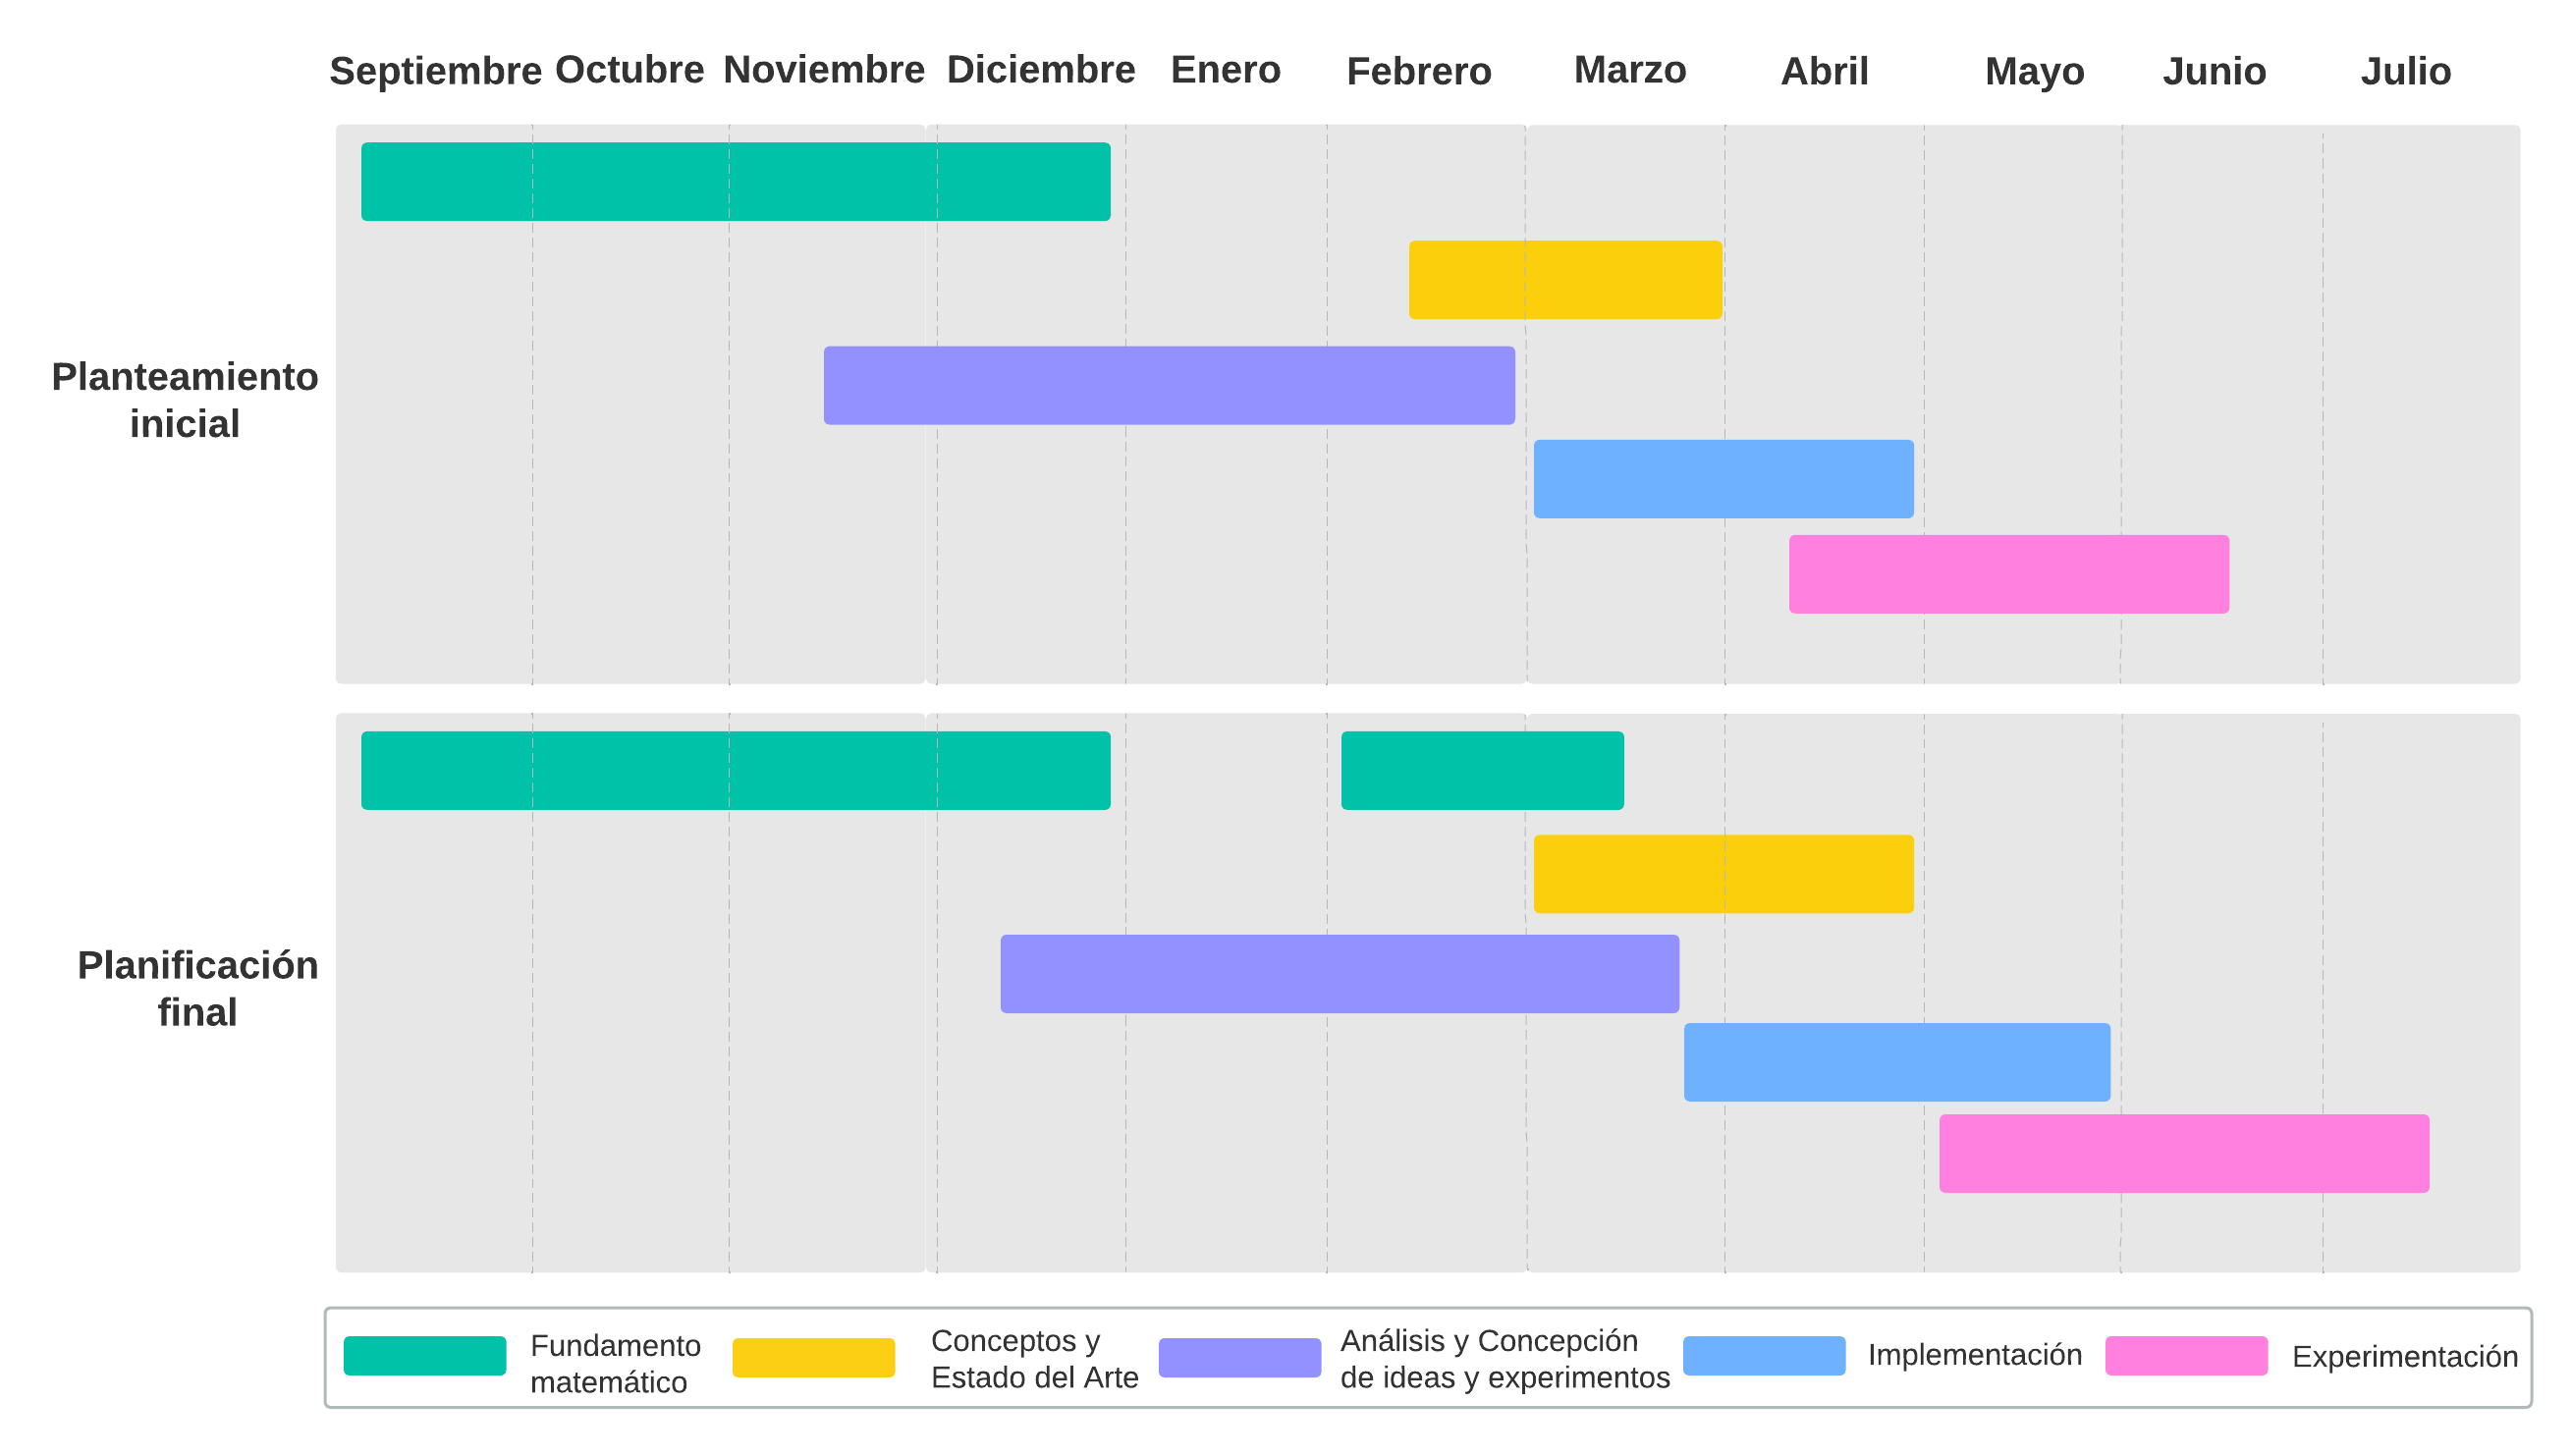
\includegraphics[width=150mm]{img/planificacion.png}
	\caption{Planificación temporal prepuesta frente a la finalmente realizada.}
	\label{fig:plan}
\end{figure}

\endinput               

% -------------------------------------------------------------------
% MAINMATTER
% -------------------------------------------------------------------
\mainmatter % activa la numeración de capítulos, resetea la numeración de las páginas y usa números arábigos

\part{Primera parte} % Dividir un TFG en partes OPCIONAL

% !TeX root = ../tfg.tex
% !TeX encoding = utf8

\chapter{Primer capítulo}\label{ch:primer-capitulo}

\section{Introducción}
Este documento es una plantilla para la elaboración de un trabajo fin de Grado siguiendo los \href{https://grados.ugr.es/matematicas/pages/infoacademica/tfg/requisitosTFG}{requisitos} de la comisión de Grado en Matemáticas de la Universidad de Granada que, a fecha de junio de 2023, son las siguientes:

\begin{itemize}
  \item La  memoria  debe  realizarse  con  un  procesador  de  texto  científico,  preferiblemente (La)TeX.
  \item La portada  debe contener  el  logo  de  la UGR,  incluir  el  título del TFG, el nombre del estudiante y especificar el grado, la facultad y el curso actual.
  \item La contraportada contendrá además el nombre del tutor o tutores.
  \item La memoria debe necesariamente incluir:
    \begin{itemize}
      \item Declaración explícita firmada en la que se asume la originalidad del trabajo, entendida en el sentido de que no ha utilizado fuentes sin citarlas debidamente. Esta declaración se puede descargar en la web del Grado.
      \item un índice detallado de capítulos y secciones,
      \item un resumen amplio en inglés del trabajo realizado (se recomienda entre 800 y 1500 palabras),
      \item una introducción en la que se describan claramente los objetivos previstos inicialmente en la propuesta de TFG, indicando si han sido o no alcanzados, los antecedentes importantes para el desarrollo, los resultados obtenidos, en su caso y las principales fuentes consultadas,
      \item una bibliografía final que incluya todas las referencias utilizadas.
    \end{itemize}
  \item Se recomienda que la extensión de la memoria sea de unas 50 páginas, sin incluir posibles apéndices.
\end{itemize}

Para generar el pdf a partir de la plantilla basta compilar el fichero \texttt{tfg.tex}. Es conveniente leer los comentarios contenidos en dicho fichero pues ayudarán a entender mejor como funciona la plantilla. 

La estructura de la plantilla es la siguiente\footnote{Los nombres de las carpetas no se han acentuado para evitar problemas en sistemas con Windows}: 
\begin{itemize}
  \item Carpeta \textbf{preliminares}: contiene los siguientes archivos
    \begin{description}
      \item[\texttt{dedicatoria.tex}] Para la dedicatoria del trabajo (opcional)
      \item[\texttt{agradecimientos.tex}] Para los agradecimientos del trabajo (opcional)
      \item[\texttt{introduccion.tex}] Para la introducción (obligatorio)
      \item[\texttt{summary.tex}] Para el resumen en inglés (obligatorio)
      \item[\texttt{tablacontenidos.tex}] Genera de forma automática la tabla de contenidos, el índice de figuras y el índice de tablas. Si bien la tabla de contenidos es conveniente incluirla, el índice de figuras y tablas es opcional. Por defecto está desactivado. Para mostrar dichos índices hay que editar este fichero y quitar el comentario a \verb+\listoffigures+ o \verb+\listoftables+ según queramos uno de los índices o los dos. En este archivo también es posible habilitar la inclusión de un índice de listados de código (si estos han sido incluidos con el paquete \texttt{listings})
  \end{description}
  El resto de archivos de dicha carpeta no es necesario editarlos pues su contenido se generará automáticamente a partir de los metadatos que agreguemos en \texttt{tfg.tex}

  \item Carpeta \textbf{capitulos}: contiene los archivos de los capítulos del TFG. Añadir tantos archivos como sean necesarios. Este capítulo es \texttt{capitulo01.tex}.

  \item Carpeta \textbf{apendices}: Para los apéndices (opcional)
  \item Carpeta \textbf{img}: Para incluir los ficheros de imagen que se usarán en el documento.
    
  \item Fichero \texttt{library.bib}: Para incluir las referencias bibliográficas en formato \texttt{bibtex}. Es útil la herramienta \href{https://www.doi2bib.org/}{doi2bib} para generar de forma automática el código bibtex de una referencia a partir de su \textsc{doi}  así como la base de datos bibliográfica \href{https://mathscinet.ams.org}{MathSciNet}. Para que una referencia aparezca en el pdf no basta con incluirla en el fichero \texttt{library.bib}, es necesario además \emph{citarla} en el documento usando el comando \verb+\cite+. Si queremos mostrar todos las referencias incluidas en el fichero \texttt{library.bib} podemos usar \verb+\cite{*}+ aunque esta opción no es la más adecuada. Se aconseja que los elementos de la bibliografía estén citados al menos una vez en el documento (y de esa forma aparecerán de forma automática en la lista de referencias).

  \item Fichero \texttt{glosario.tex}: Para incluir un glosario en el trabajo (opcional). Si no queremos incluir un glosario deberemos borrar el comando \verb+% !TeX root = ../tfg.tex
% !TeX encoding = utf8

\chapter*{Glosario}
\addcontentsline{toc}{chapter}{Glosario} % Añade el glosario a la tabla de contenidos

La inclusión de un glosario es opcional.

Archivo: \texttt{glosario.tex}

\begin{description} 
  \item[$\mathbb{R}$] Conjunto de números reales.

  \item[$\mathbb{C}$] Conjunto de números complejos.

  \item[$\mathbb{Z}$] Conjunto de números enteros.
\end{description}
\endinput
+ del fichero \texttt{tfg.tex} y posteriormente borrar el fichero \texttt{glosario.tex}

   \item Fichero \texttt{tfg.tex}: El documento maestro del TFG que hay que compilar con \LaTeX\ para obtener el pdf. En dicho documento hay que cambiar la \emph{información del título del \textsc{tfg} y el autor así como los tutores}.
\end{itemize}



\section{Elementos del texto}

En esta sección presentaremos diferentes ejemplos de los elementos de texto básico. Conviene consultar el contenido de \texttt{capitulos/capitulo01.tex} para ver cómo se han incluido.

\subsection{Listas}
En \LaTeX\ tenemos disponibles los siguientes tipos de listas:

Listas enumeradas:
\begin{enumerate}
  \item item 1
  \item item 2
  \item item 3
\end{enumerate}

Listas no enumeradas
\begin{itemize}
  \item item 1
  \item item 2
  \item item 3
  \end{itemize}

Listas descriptivas
\begin{description}
  \item[termino1] descripción 1
  \item[termino2] descripción 2
\end{description}
  
\subsection{Tablas y figuras}

En la \autoref{tb:ejemplo-tabla} o la \autoref{fig:logo-ugr} podemos ver\ldots

\begin{table}[htpb]
  \centering
  \begin{tabular}{ccc} \toprule
    \multicolumn{2}{c}{Agrupados} \\ \cmidrule(r){1-2}
    cabecera & cabecera & cabecera          \\ \midrule
    elemento & elemento & elemento          \\ 
    elemento & elemento & elemento          \\ 
    elemento & elemento & elemento          \\ \bottomrule
  \end{tabular}
  \caption{Ejemplo de tabla}
  \label{tb:ejemplo-tabla}
\end{table}

\begin{figure}[htpb]
  \centering
  
\includegraphics[width=0.5\textwidth]{logo-ugr}
  \caption{Logotipo de la Universidad de Granada}
  \label{fig:logo-ugr}
\end{figure}

\section{Entornos matemáticos}\label{sec:entornos-matematicos}

La plantilla tiene definidos varios entornos matemáticos cuyo nombre es el mismo omitiendo los acentos. Así, para incluir una \emph{proposición} usaríamos:

\begin{verbatim}
\begin{proposicion}
texto de la proposición
\end{proposicion} 
\end{verbatim}

Ver el código fuente del archivo \texttt{capitulo01.tex} para el resto de ejemplos.

\begin{teorema}\label{thm:teorema}
Esto es un ejemplo de teorema.
\end{teorema}

\begin{proposicion}
Ejemplo de proposición
\end{proposicion}

\begin{lema}
Ejemplo de lema
\end{lema}

\begin{corolario}
Ejemplo de corolario
\end{corolario}

\begin{definicion}
Ejemplo de definición
\end{definicion}

\begin{observacion}
Ejemplo de observación
\end{observacion}

Adicionalmente está definido el entorno \texttt{teorema*} que permite incluir un teorema sin numeración:

\begin{teorema*}[Fórmula de Gauß-Bonnet]
  Sea $S$ una superficie compacta y $K$ su curvatura de Gauß. Entonces
\begin{equation}
  \int_S K = 2\pi\chi(S)
\end{equation}
donde $\chi(S)$ es la característica de Euler de $S$.
\end{teorema*}

Las fórmulas matemáticas se escriben entre símbolos de dólar \$ si van en línea con el texto o bien usando el entorno%
\footnote{
  También es posible delimitar una ecuación mediante los comandos \texttt{$\backslash$[} y \texttt{$\backslash$]} pero éstas nunca llevarán numeración aunque añadamos una etiqueta y las referenciemos (ver \autoref{sec:referencias}).
} 
\texttt{equation} cuando queremos que se impriman centradas en una línea propia, como el siguiente ejemplo
\begin{equation}\label{eq:identidad-pitagorica}
  \cos^2 x + \sin^2 x = 1.
\end{equation}


Gracias al paquete \texttt{mathtools}, las ecuaciones escritas dentro del entorno \texttt{equation} llevarán numeración de forma automática si son referenciadas  en cualquier parte del documento (por ejemplo la identidad Pitagórica~\eqref{eq:identidad-pitagorica}, ver el código de los dos anteriores ejemplos y la \autoref{sec:referencias} para más información sobre referencias cruzadas en el documento).




\section{Referencias a elementos del texto}\label{sec:referencias}

Para las referencias a los elementos del texto (secciones, capítulos, teoremas,\ldots) se procede de la siguiente manera:
\begin{itemize}
  \item Se \emph{marca} el elemento (justo antes del mismo si se trata de un capítulo o sección o en el interior del \emph{entorno} en otro caso), mediante el comando \verb+\label{+\emph{etiqueta}\verb+}+, donde \emph{etiqueta} debe ser un identificador único.
  \item Para crear una referencia al elemento en cualquier otra parte del texto se usa el comando \verb+\ref{+\emph{etiqueta}\verb+}+ (únicamente imprime la numeración asociada a dicho elemento, por ejemplo \ref{ch:primer-capitulo} o \ref{thm:teorema}) o bien \verb+\autoref{+\emph{etiqueta}\verb+}+ (imprime la numeración del elemento así como un texto previo indicando su tipo, por ejemplo \autoref{ch:primer-capitulo} o \autoref{thm:teorema})
\end{itemize}




\section{Bibliografía e índice}

Esto es un ejemplo de texto en un capítulo. Incluye varias citas tanto a libros~\cite{Aigner2018}, artículos de investigación~\cite{Euler1985}, recursos online~\cite{EulerWiki} (páginas web), tesis~\cite{CitekeyPhdthesis}, trabajo fin de máster~\cite{CitekeyMastersthesis}, trabajo fin de grado~\cite{CiteKeyBachelorsthesis} así como artículos sin publicar (preprints) \cite{castroinfantes2022conjugate} (en estos últimos usar el campo \texttt{note} para añadir la información relevante). Ver el fichero \texttt{library.bib} para las distintas plantillas. 


\endinput

% Añadir tantos capítulos como sea necesario
% !TeX root = ../tfg.tex
% !TeX encoding = utf8

\chapter{Símplices y complejos simpliciales}

\section{Símplices}

INTRO

\begin{definicion}
	Sea $\{a_0, \dots, a_n\}$ un conjunto de puntos en $\mathbb{R}^N$. 
	Diremos que dicho conjunto es \textbf{afínmente independiente} si 
	para cualesquiera $t_i \in \mathbb{R}$, las ecuaciones
	\[ \sum_{i=0}^{n}t_i=0 \quad \text{y} \quad \sum_{i=0}^{n}t_ia_i=0 \]
	implican que $t_0 = t_1 = \dots = t_n$.
\end{definicion}

TEXTO

\begin{definicion}
	Sea $\{a_0, \dots, a_n\}$ un conjunto de puntos afínmente independiente. 
	Definimos el \textbf{n-plano} $P$ generado por $\{a_0, \dots, a_n\}$ como
	el conjunto de puntos $x \in \mathbb{R}^N$ tales que
	\[ x = a_0 + \sum_{i=1}^{n}t_i(a_i - a_0) \]
	para algunos $t_1, \dots, t_n \in \mathbb{R}$. Diremos entonces que $P$ es el 
	plano que pasa por $a_0$ paralelo a los vectores $a_i - a_0$, $i \in \{1, \dots, n\}$.
\end{definicion}

\begin{definicion}
	Def de aplicación afín.
\end{definicion}

\begin{definicion}
	Sea $\{a_0, \dots, a_n\}$ un conjunto de puntos afínmente independiente en 
	$\mathbb{R}^N$. Definimos el \textbf{símplice} $\sigma = [a_0, \dots, a_n]$ 
	generado por $a_0, 	\dots, a_n$ como el conjunto de todos los $x \in \mathbb{R}^N$ 
	tales que
	\[ x=\sum_{i=0}^{n}t_ia_i \quad \text{y} \quad \sum_{i=0}^{n}t_i=1 \]
	con $t_i \geq 0$, $i \in \{1, \dots, n\}$.
\end{definicion}
Los coeficientes $t_i$ están determinados de manera única por el punto $x$. Al conjunto 
$\{t_0, \dots, t_n \}$ lo llamamos las \textbf{coordenadas baricéntricas} de $\sigma$
con respecto a $a_0, \dots, a_n$.

Los puntos $a_0, \dots, a_n$ que generan $\sigma$ los llamaremos \textbf{vértices} de $\sigma$
y al número $n$ lo llamaremos la \textbf{dimensión} de $\sigma$.

\begin{definicion}
	Sea $\sigma=[a_0, \dots, a_n]$ un símplice. Una \textbf{cara} de $\sigma$ será cualquier
	símplice generado por un subconjunto de $\{a_0, \dots, a_n\}$.
\end{definicion}
En particular, la cara de $\sigma$ generada por $a_0, \dots, a_{i-1}, a_{i+1}, \dots, a_n$ la 
llamamos la \textbf{cara opuesta} de $a_i$, $i \in \{0, \dots, n\}$. Las caras de $\sigma$ 
diferentes de $\sigma$ diremos que son \textbf{caras propias} de $\sigma$ y la unión de todas ellas la 
llamaremos el \textbf{borde} de $\sigma$. Finalmente, definimos el \textbf{interior} de $\sigma$
como el conjunto de puntos de $\sigma$ que no pertenecen a su borde.

\section{Complejos simpliciales}

\endinput
%--------------------------------------------------------------------
% FIN DEL CAPÍTULO. 
%--------------------------------------------------------------------


\cleardoublepage\part{Segunda parte}
% !TeX root = ../tfg.tex
% !TeX encoding = utf8

\chapter{Ejemplo de capítulo}

\section{Primera sección}

Este fichero \texttt{capitulo-ejemplo.tex} es una plantilla para añadir capítulos al \textsc{tfg}. Para ello, es necesario:
\begin{itemize}
  \item Crear una copia de este fichero \texttt{capitulo-ejemplo.tex} en la carpeta \texttt{capitulos} con un nombre apropiado (p.e. \texttt{capitulo01.tex}).
  \item Añadir el comando \texttt{$\backslash$input\{capitulos/capitulo01\}} en el fichero principal \texttt{tfg.tex} donde queremos que aparezca dicho capítulo.
\end{itemize}


\endinput
%--------------------------------------------------------------------
% FIN DEL CAPÍTULO. 
%--------------------------------------------------------------------


% -------------------------------------------------------------------
% APPENDIX: Opcional
% -------------------------------------------------------------------

\appendix % Reinicia la numeración de los capítulos y usa letras para numerarlos
\pdfbookmark[-1]{Apéndices}{appendix} % Alternativamente podemos agrupar los apéndices con un nuevo \part{Apéndices}

% !TeX root = ../tfg.tex
% !TeX encoding = utf8

\chapter{Ejemplo de apéndice}\label{ap:apendice1}

Los apéndices son opcionales.

Este fichero \texttt{apendice-ejemplo.tex} es una plantilla para añadir apéndices al \textsc{tfg}. Para ello, es necesario:
\begin{itemize}
  \item Crear una copia de este fichero \texttt{apendice-ejemplo.tex} en la carpeta \texttt{apendices} con un nombre apropiado (p.e. \texttt{apendice01.tex}).
  \item Añadir el comando \texttt{$\backslash$input\{apendices/apendice01\}} en el fichero principal \texttt{tfg.tex} donde queremos que aparezca dicho apéndice (debe de ser después del comando \texttt{$\backslash$appendix}).
\end{itemize}

\endinput
%------------------------------------------------------------------------------------
% FIN DEL APÉNDICE. 
%------------------------------------------------------------------------------------

% Añadir tantos apéndices como sea necesario 

% -------------------------------------------------------------------
% GLOSARIO: Opcional
% -------------------------------------------------------------------

% !TeX root = ../tfg.tex
% !TeX encoding = utf8

\chapter*{Glosario}
\addcontentsline{toc}{chapter}{Glosario} % Añade el glosario a la tabla de contenidos

La inclusión de un glosario es opcional.

Archivo: \texttt{glosario.tex}

\begin{description} 
  \item[$\mathbb{R}$] Conjunto de números reales.

  \item[$\mathbb{C}$] Conjunto de números complejos.

  \item[$\mathbb{Z}$] Conjunto de números enteros.
\end{description}
\endinput
 

% -------------------------------------------------------------------
% BACKMATTER
% -------------------------------------------------------------------

\backmatter % Desactiva la numeración de los capítulos
\pdfbookmark[-1]{Referencias}{BM-Referencias}

% BIBLIOGRAFÍA
%-------------------------------------------------------------------

\bibliographystyle{alpha-es} 
\begin{small} 
  \bibliography{library.bib}
\end{small}


\end{document}
